\documentclass[UTF8]{ctexart}
\usepackage{amsmath}
\usepackage{ltablex}
\usepackage{tabularx}
\usepackage{forloop}
\usepackage{xstring}
\usepackage{ifthen}
\usepackage{calc}
\usepackage{color}
\usepackage[margin=1in]{geometry}

% \usepackage{hyperref}
% \hypersetup{pdftex,colorlinks=true,allcolors=blue}
% \usepackage{hypcap}

\usepackage[]{hyperref}
\hypersetup{
    pdftitle={FSI Cantonese - new format},
    pdfauthor={Foreign Services Institute},
    pdfsubject={FSI Cantonese},
    bookmarksnumbered=true,
    bookmarksopen=true,
    bookmarksopenlevel=1,
    % colorlinks=true,
    pdfstartview=Fit,
    pdfpagemode=UseOutlines,
    pdfpagelayout=TwoPageRight
}

% Make font larger
\setCJKmainfont[Scale=1.5]{STSong}

% Input custom functions

%%%%%%%%%%%%%%%%%%%%%%%%%%%%%%%%%%%%%%%%%%%%%%%%%%%%%%%%%%%%%%%%%%%%%%%%%%%%%%%%

% Jyutping formatting which takes as input a string like xxxxNxxxxN and produces
% a string where the N are superscripted.
% \jping{ji4gaa1}
%
% @param string of the format xxxxNxxxxN
\newcounter{jpingStart}
\newcounter{jpingEnd}
\newcounter{jpingIndex}
\newcounter{jpingLength}
\newcounter{jpingLengthPlusOne}
\newcommand{\jping}[1]{%
    % NOTE: for single use, this would work, but we need to split...
    % \StrGobbleRight{#1}{1}\textsuperscript{\StrRight{#1}{1}}%
    % Get length of text
    \StrLen{#1}[\jpingLength]%
    \setcounter{jpingLengthPlusOne}{\jpingLength + 1}%
    % Set start of text
    \setcounter{jpingStart}{1}%
    \setcounter{jpingEnd}{0}%
    % Loop over each char
    \forloop{jpingIndex}{1}{\value{jpingIndex} < \arabic{jpingLengthPlusOne}}{%
        % Get char
        \StrChar{#1}{\arabic{jpingIndex}}[\jpingChar]%
        % If numeric, then handle
        % NOTE: include 7 for high falling examples
        \IfSubStr{1234567*}{\jpingChar}{%
            \text{\textsuperscript{\jpingChar}}%
        }{%
            \text{\jpingChar}%
        }%
    }%
}%

%%%%%%%%%%%%%%%%%%%%%%%%%%%%%%%%%%%%%%%%%%%%%%%%%%%%%%%%%%%%%%%%%%%%%%%%%%%%%%%%

% Variables for dtext
\newcounter{dtextStart}
\newcounter{dtextEnd}
\newcounter{dtextIndex}
\newcounter{dtextSubWordPlusOne}
\newcounter{dtextLength}
\newcounter{dtextLengthPlusOne}
\newcounter{dtextSubWord}
\newcounter{dtextNormal}

% Double text, meaning cantonese characters on top, and jyutping ont he bottom.
% The characters and jyutping will be grouped by spaces, with punctuation
% (including chinese punctuation), correctly ignored and skipped. Uses \jping
% for each jyutping group.
%
% Test cases
% \dtext{而家 我 問 你,你 答 我。}{ji4gaa1 ngo5 man6 nei5 nei5 daap3 ngo5}\\
% \dtext{而家 我 問 你,你 答 我。X}{ji4gaa1 ngo5 man6 nei5 nei5 daap3 ngo5 w}\\
% \dtext{而家}{ji4gaa1}\\
% \dtext{而家 我 問 你,你 答 我。a}{ji4gaa1 ngo5 man6 nei5 nei5 daap3 ngo5 -}\\
% \dtext{而家 我 問 你,你 答 我。X b}{ji4gaa1 ngo5 man6 nei5 nei5 daap3 ngo5 w -}\\
% \dtext{而家}{-}\\
% \dtext{而家。。。}{ji4gaa1}\\
% \dtext{而家 我 問 你,,你 答 我。。。}{ji4gaa1 ngo5 man6 nei5 nei5 daap3 ngo5}\\
% TODO: Mode: top only, top and bottom, bottom only, top and bottom white
%
% @param cantonese characters
% @param jyutping
\newcommand{\dtext}[2]{%
    % Get length of text
    \StrLen{#1}[\dtextLength]%
    \setcounter{dtextSubWord}{0}%
    \setcounter{dtextNormal}{0}%
    \setcounter{dtextLengthPlusOne}{\dtextLength + 1}%
    % Count number of spaces
    \StrCount{#2}{ }[\dtextSpaces]
    % Set start of word
    \setcounter{dtextStart}{1}%
    \setcounter{dtextEnd}{0}%
    % Loop over each char
    \forloop{dtextIndex}{1}{\value{dtextIndex} < \arabic{dtextLengthPlusOne}}{%
        % Get char
        \StrChar{#1}{\arabic{dtextIndex}}[\dtextChar]%
        % If special, then handle
        % https://en.wikipedia.org/wiki/Chinese_punctuation
        \IfSubStr{; 。「」﹁﹂"、‧《》〈〉﹏…——~,?;,!-?}{\dtextChar}{%
            % End of word
            \StrMid{#1}{\arabic{dtextStart}}{\arabic{dtextEnd}}[\textOver]%
            \stepcounter{dtextEnd}%
            \setcounter{dtextStart}{\arabic{dtextEnd}}%
            \stepcounter{dtextStart}%
            \ifthenelse{\equal{\arabic{dtextNormal}}{\string 0}}{%
                % No characters! Just print this one and continue
            }{%
                % Add subtext
                \ifthenelse{\equal{\arabic{dtextSubWord}}{\string 0}}{%
                    % Handle first case
                    \StrCut[1]{#2}{ }{\textUnder}{\rightpart}%
                }{%
                    % Handle last case
                    \ifthenelse{\equal{\arabic{dtextSubWord}}{\dtextSpaces}}{%
                        % IF ALL LAST .... then wont be caught...
                        \StrCut[\arabic{dtextSubWord}]{#2}{ }{\leftpart}{\textUnder}%
                    }{% Handle middle case
                        \setcounter{dtextSubWordPlusOne}{\arabic{dtextSubWord} + 1}%
                        \StrBetween[\arabic{dtextSubWord},\arabic{dtextSubWordPlusOne}]{#2}{ }{ }[\textUnder]%
                    }%
                }%
                % Handle ignore
                \ifthenelse{\equal{\textUnder}{\string -}}{%
                    \text{\textOver}%
                }{%
                    $\underset{\jping{\textUnder}}{\text{\textOver}}$%
                }%
                % \text{[\textUnder][\textOver][\dtextChar]}
                \stepcounter{dtextSubWord}%
                \setcounter{dtextNormal}{0}%
            }%
            % Enable wrapping with stupid spaces...
            \ifthenelse{\equal{\dtextChar}{ }}{%
                \text{} %
            }{%
                \text{\dtextChar}%
            }%
        }{%
            % Not end of word
            \stepcounter{dtextEnd}%
            \stepcounter{dtextNormal}%
            % Handle last not being special
            \ifthenelse{\equal{\arabic{dtextIndex}}{\dtextLength}}{%
                % End of word
                \StrMid{#1}{\arabic{dtextStart}}{\arabic{dtextEnd}}[\textOver]%
                \stepcounter{dtextEnd}%
                \setcounter{dtextStart}{\arabic{dtextEnd}}%
                \stepcounter{dtextStart}%
                % Special case of single word
                \ifthenelse{\equal{\arabic{dtextSubWord}}{\string 0}}{%
                    % FIXME: lazy...
                    \StrMid{#2}{0}{9999}[\textUnder]%
                }{%
                    \StrCut[\arabic{dtextSubWord}]{#2}{ }{\leftpart}{\textUnder}%
                }%
                % Handle ignore
                \ifthenelse{\equal{\textUnder}{\string -}}{%
                    \text{\textOver}%
                }{%
                    $\underset{\jping{\textUnder}}{\text{\textOver}}$%
                }%
            }{%
            }%
        }%
    }%
}

%%%%%%%%%%%%%%%%%%%%%%%%%%%%%%%%%%%%%%%%%%%%%%%%%%%%%%%%%%%%%%%%%%%%%%%%%%%%%%%%

% Create two column, auto numbered classroom phrases, ie
% \classroomPhrases{
%   {而家踏幾呀}{ready yet}
%   {而家踏幾呀}{ready yet}
%   {\dtext{而家踏幾呀}{ji4 gaa1 daap3 gei2 aa3}}{ready yet}
% }
%
% @param array of tuples
\newcommand*{\classroomPhrases}[1]{%
    \setcounter{classroomPhraseCounter}{1}
    \relax
    \renewcommand{\arraystretch}{2}
    \noindent\begin{tabularx}{\linewidth}{l X l X}
    \classroomPhrase#1\relax\relax
    \end{tabularx}
    \renewcommand{\arraystretch}{1}
}
\newcounter{classroomPhraseCounter}
% Helper method for classroomPhrases
\newcommand{\classroomPhrase}[2]{%
    \ifx\relax#1\\\empty%
    \else%
    \noindent\arabic{classroomPhraseCounter}. & #1 & \arabic{classroomPhraseCounter}. & #2\\\relax%
    \stepcounter{classroomPhraseCounter}%
    \expandafter\classroomPhrase%
    \fi%
}

%%%%%%%%%%%%%%%%%%%%%%%%%%%%%%%%%%%%%%%%%%%%%%%%%%%%%%%%%%%%%%%%%%%%%%%%%%%%%%%%

% Create three column, auto numbered vocabulary list, ie
% \vocabularyChecklist{
%   {A}{ex}{oh}
%   {Chahn}{sur}{Chan}
%   {deimyjhyu}{ph}{Excuse me; I beg your pardon; I'm sorry}
%   {而家踏幾呀}{abc}{ready yet}
% }
%
% @param array of triples
\newcommand*{\vocabularyChecklist}[1]{%
    \setcounter{vocabularyChecklistCounter}{1}
    \relax
    \renewcommand{\arraystretch}{2}
    \noindent\begin{tabularx}{\linewidth}{r l r X}
    \vocabularyEntry#1\relax\relax\relax
    \end{tabularx}
    \renewcommand{\arraystretch}{1}
}
\newcounter{vocabularyChecklistCounter}
% Helper method for vocabularyChecklist
\newcommand{\vocabularyEntry}[3]{%
    \ifx\relax#1\\\empty%
    \else%
    \arabic{vocabularyChecklistCounter}. & #1 & #2: & #3\\\relax%
    \stepcounter{vocabularyChecklistCounter}%
    \expandafter\vocabularyEntry%
    \fi%
}

%%%%%%%%%%%%%%%%%%%%%%%%%%%%%%%%%%%%%%%%%%%%%%%%%%%%%%%%%%%%%%%%%%%%%%%%%%%%%%%%

% Create a drill
% NOTE: does not use simple nested stuff, due to ifthenelse and multicolumn
% errors on omit

% \drillExample{
%    \drillExampleEntry {T} {\dtext{李 太,早晨}{lei5 taai2 zou2san4}} {Good morning, Mrs. Lee.}
%    \drillExampleEntry {S} {\dtext{李 太,再見}{lei5 taai2 zoi3gin3}} {Goodbye, Mrs. Lee.}
% }
% \drillExample{
%    \drillExampleEntrySub {T} {\dtext{李 太,早晨}{lei5 taai2 zou2san4}} {Good morning, Mrs. Lee.} {\dtext{陳}{can4}}
%    \drillExampleEntry {S} {\dtext{陳 太,再見}{can4 taai2 zoi3gin3}} {Good morning, Mrs. Chan.}
% }
\newcommand*{\drillExample}[1]{%
    \begin{minipage}{\linewidth}
        Ex:
        \relax
        \renewcommand{\arraystretch}{2}
        \noindent\begin{tabularx}{\linewidth}{l X | l X}
        #1\relax\relax
        \end{tabularx}
        \renewcommand{\arraystretch}{1}
    \end{minipage}
}

% Example drill entry
%
% @param speaker
% @param left
% @param right
\newcommand{\drillExampleEntry}[3]{%
    #1: & #2 & #1: & #3 \\%
}%

% Example drill entry translation
%
% @param left
% @param right
\newcommand{\drillExampleEntryTrans}[2]{%
    & #1 & & #2 \\%
}%

% Example drill entry with substitution
%
% @param speaker
% @param left
% @param right
% @param substitution
\newcommand{\drillExampleEntrySub}[4]{%
    #1. & #2 & #1. & #3 \\%
    & / #4 / & & \\%
}%

% \drill{
%    \drillEntrySub {1} {\dtext{陳 太,早晨}{can4 taai2 zou2san4}} {\dtext{李 太,早晨}{lei5 taai2 zou2san4}} {\dtext{李}{lei5}}
%    \drillEntry {2} {\dtext{劉 生,早晨}{lau4 saang1 zou2san4}}{\dtext{劉 生,再見} {lau4 saang1 zoi3gin3}}
%    \drillEntryTrans {Good morning, Mr. Lau.} {}
% }
\newcommand*{\drill}[1]{%
    \renewcommand{\arraystretch}{2}
    \noindent\begin{tabularx}{\linewidth}{l l | l l}
    #1\relax\relax
    \end{tabularx}
    \renewcommand{\arraystretch}{1}
}

% Drill entry
%
% @param number
% @param left
% @param right
\newcommand{\drillEntry}[3]{%
    \IfSubStr{1234567890}{#1}{#1.}{} & #2 & \IfSubStr{1234567890}{#1}{#1.}{} & #3 \\%
}%

% Drill entry translation
%
% @param left
% @param right
\newcommand{\drillEntryTrans}[2]{%
    & #1 & & #2 \\%
}%

% Drill entry with substitution
%
% @param number
% @param left
% @param right
\newcommand{\drillEntrySub}[4]{%
    #1. & #2 & #1. & #3 \\%
    & / #4 / & & \\%
}%

\newcommand*{\convDrill}[1]{%
    \renewcommand{\arraystretch}{2}
    \noindent\begin{tabularx}{\linewidth}{l l X | l l X}
    #1\relax\relax
    \end{tabularx}
    \renewcommand{\arraystretch}{1}
}

\newcommand{\convDrillEntry}[4]{%
    \IfSubStr{1234567890}{#1}{#1.}{} & #2: & #3 & \IfSubStr{1234567890}{#1}{#1.}{} & #2: & #4 \\%
}%


%%%%%%%%%%%%%%%%%%%%%%%%%%%%%%%%%%%%%%%%%%%%%%%%%%%%%%%%%%%%%%%%%%%%%%%%%%%%%%%%

% Create an audio tag
%
% @param tape side A/B
% @param timestamp in 0:00 format
\newcommand{\audioTag}[2]{%
    #1 $\triangleright$ #2%
}%

\newcommand{\subsText}[1]{%
    /#1/%
}

%%%%%%%%%%%%%%%%%%%%%%%%%%%%%%%%%%%%%%%%%%%%%%%%%%%%%%%%%%%%%%%%%%%%%%%%%%%%%%%%

% Create a converstation
% NOTE: does not use simple nested stuff, due to ifthenelse and multicolumn
% errors on omit
%
% \conversation{
%   %
%   \convBackground{(At the beginning of class in the morning)}
%   %
%   \convExplanation{\dtext{學生}{hok6saang1}}{student}
%   %
%   \cspeaker{\dtext{學生}{hok6saang1}}
%   \cbline{\dtext{何}{ho4}}{Ho, surname}
%   \cbline{\dtext{生}{saang1}}{Mr.}
%   \cbline{\dtext{何 生}{ho4 saang1}}{Mr. Ho}
%   \cbline{\dtext{早晨}{zou2san4}}{good morning}
%   \cfline{\dtext{何 生 早晨}{ho4 saang1 zou2san4}}{Good morning, Mr. Ho.}
%   \convExplanation{\dtext{先生}{sin1saang1}}{teacher}
%   %
%   \cspeaker{\dtext{先生}{sin1saang1}}
%   \cbline{\dtext{李}{lei5}}{Lee, surname}
%   \cbline{\dtext{太}{taai2}}{Mrs.}
%   \cbline{\dtext{李 太}{lei5 taai2}}{Mrs. Lee}
%   \cfline{\dtext{李 太 早晨。}{lei5 taai2 zou2san4}}{Good morning, Mrs. Lee.}
%   %
%   \convBackground{(At the end of the day, the students are leaving class.)}
%   %
% }
% @param table rows
\newcommand*{\conversation}[1]{%
    \relax
    \renewcommand{\arraystretch}{2}
    \noindent\begin{tabularx}{\linewidth}{X | X}
    #1\relax\relax
    \end{tabularx}
    \renewcommand{\arraystretch}{1}
}

% A line for a speaker change
%
% @param speaker name
\newcommand{\cspeaker}[1]{%
    \multicolumn{2}{c}{\textbf{\underline{#1}}} \\%
}%

% A line for a double width row (background information)
%
% @param text
\newcommand{\convBackground}[1]{%
    \multicolumn{2}{c}{#1} \\%
}%

% Buildup line
%
% @param left right
\newcommand{\cbline}[2]{%
    \indent #1 & \indent #2\\%
}%

% Full conversation line after a buildup
%
% @param left right
\newcommand{\cfline}[2]{%
    #1 & #2\\%
}%

% Additional conversation line (i.e. word explanation)
%
% @param left right
\newcommand{\convExplanation}[2]{%
    \indent #1 & \indent #2\\%
}%

\newcommand*{\listeningConversation}[1]{%
    \relax
    \renewcommand{\arraystretch}{2}
    \noindent\begin{tabularx}{\linewidth}{l l}
    #1\relax\relax
    \end{tabularx}
    \renewcommand{\arraystretch}{1}
}

\newcommand{\lcEntry}[2]{%
    #1: & #2\\%
}%

%%%%%%%%%%%%%%%%%%%%%%%%%%%%%%%%%%%%%%%%%%%%%%%%%%%%%%%%%%%%%%%%%%%%%%%%%%%%%%%%

% Translater note
%
% @param text
\newcommand{\tnote}[1]{%
    \underline{Translation Note}: #1%
}

% TODO note
%
% @param text
\newcommand{\todo}[1]{%
    \textbf{\underline{TODO}}: #1%
}

\begin{document}

\title{FSI Cantonese - new format}
\author{Foreign Services Institute}

\maketitle

\tableofcontents

\newpage
Translator notes:
\begin{itemize}
    \item The original FSI cantonese uses yale romanization with 7 tones. This translation uses jyupting with 6 tones.
    \item This is a work in progress
\end{itemize}

% Lesson 00
\section{Preface}
\todo{copy}

\section{Introduction}
\todo{copy}

\section{Objectives of the course}
\todo{copy}

\section{Procedure}
\todo{copy}

\section{Suggestions for Further Practice}
\todo{copy}

\section{Symbols used in this text}
\todo{copy}

% Lesson 01
\newpage
\section{Lesson 1}

\subsection{Classroom Phrases}

\audioTag{A}{0:05}

The instructor will address you in Cantonese from the first day of class. The following are some instructions which you should learn to respond to. Look at your books while the instructor reads the phrases the first time. Then close your books, and the teacher will give the phrases several more times, using gestures to help you understand. Repease the phrases after him, mimicking his movements as well as his voice, to help you absorb the rhythm and meaning.

\classroomPhrases{
	{\dtext{而家 你哋 聽住 我 講。}{ji4gaa1 nei5dei6 teng1zyu6 ngo5 gong2}}{Now you (plu.) listen while I speak. (i.e., listen, but you don't repeat)}
	{\dtext{而家 我 講,你哋 跟住 我 講。}{ji4gaa1 ngo5 gong2 nei5dei6 gan1zyu6 ngo5 gong2}}{Now I'll speak and you repeat after me.}
	{\dtext{x 本書,x 啲書。}{? bun2syu1, ? di1syu1}}{Close the book, close the books.}
	{\dtext{打開 本 書, 打開 啲 書。}{daa2hoi1 bun2 syu1, daa2hoi1 di1 syu1}}{Close the book, close the books.}
	{\dtext{而家 一 個 一 個 講。}{ji4gaa1 jat1 go3 jat1 go3 gong2}}{Now recite one by one.}
	{\dtext{一齊 講。}{jat1cai4 gong2}}{Recite all together.}
	{\dtext{而家 一齊 跟住 我 講。}{ji4gaa1 jat1cai4 gan1zyu6 ngo5 gong2}}{Now all together repeat after me.}
	{\dtext{再 講 一 次。}{zoi3 gong2 jat1 ci3}}{Say it again.}
	{\dtext{唔好 睇 書。}{m4hou2 tai2 syu1}}{Don't look at your book(s).}
}
\subsection{Basic Conversation}

\audioTag{A}{1:43}

%%%%%%%%%%%%%%%%%%%%%%%%%%%%%%%%%%%%%%%%
\subsubsection{Buildup}

\conversation{
    %
    \convBackground{(At the beginning of class in the morning)}
    %
    \convExplanation{\atext{學生}}{student}
    %
    \cspeaker{\atext{學生}}
    \cbline{\atext{何}}{Ho, surname}
    \cbline{\atext{生}}{Mr.}
    \cbline{\atext{何 生}}{Mr. Ho}
    \cbline{\atext{早晨}}{good morning}
    \cfline{\atext{何 生 早晨}}{Good morning, Mr. Ho.}
    \convExplanation{\atext{先生}}{teacher}
    %
    \cspeaker{\atext{先生}}
    \cbline{\atext{李}}{Lee, surname}
    \cbline{\atext{太}}{Mrs.}
    \cbline{\atext{李 太}}{Mrs. Lee}
    \cfline{\atext{李 太 早晨。}}{Good morning, Mrs. Lee.}
    %
    \cspeaker{\atext{學生}}
    \cbline{\atext{對唔住}}{excuse me}
    \cbline{\atext{我}}{I}
    \cbline{\atext{係}}{am, is, are}
    \cbline{\atext{唔}}{not}
    \cbline{\atext{唔係}}{am not, is not, are not}
    \cbline{\atext{我 唔係 李 太。}}{I'm not Mrs. Lee.}
    \cfline{\atext{對唔住,我 唔係 李 太。}}{Excuse me, I'm not Mrs. Lee.}
    %
    \cbline{\atext{姓}}{have the surname}
    \cbline{\atext{陳}}{Chan}
    \cfline{\atext{我 姓 陳。}}{My name is Chan.}
    %
    \cspeaker{\atext{先生}}
    \cbline{\atext{小姐}}{Miss; unmarried woman}
    \cbline{\atext{陳 小姐}}{Miss Chan}
    \cbline{\atext{呀}{aa3}}{Oh, Ah, a mild exclamation}
    \cfline{\atext{呀,對唔住 陳 小姐。}}{Oh, excuse me, Miss Chan.}
    %
    \cspeaker{\atext{學生}}
    \cfline{\atext{唔緊要}}{That's all right. \underline{OR} It doesn't matter.}
    %
    \convBackground{(At the end of the day, the students are leaving class.)}
    %
    \cspeaker{\atext{學生}}
    \cfline{\atext{再見}}{Goodbye.}
    %
    \cspeaker{\atext{先生}}
    \cfline{\atext{再見}}{Goodbye.}
}

%%%%%%%%%%%%%%%%%%%%%%%%%%%%%%%%%%%%%%%%
\subsubsection{Recapitulation}

\audioTag{A}{7:30}

\conversation{
    %
    \convBackground{(At the beginning of class in the morning)}
    %
    \cspeaker{\atext{學生}}
    \cfline{\atext{何 生 早晨}}{Good morning, Mr. Ho.}
    %
    \cspeaker{\atext{先生}}
    \cfline{\atext{李 太 早晨。}}{Good morning, Mrs. Lee.}
    %
    \cspeaker{\atext{學生}}
    \cfline{\atext{對唔住,我 唔係 李 太。}}{Excuse me, I'm not Mrs. Lee.}
    %
    \cfline{\atext{我 姓 陳。}}{My name is Chan.}
    %
    \cspeaker{\atext{先生}}
    \cfline{\atext{呀,對唔住 陳 小姐。}}{Oh, excuse me, Miss Chan.}
    %
    \cspeaker{\atext{學生}}
    \cfline{\atext{唔緊要}}{That's all right. \underline{OR} It doesn't matter.}
    %
    \convBackground{(At the end of the day, the students are leaving class.)}
    %
    \cspeaker{\atext{學生}}
    \cfline{\atext{再見}}{Goodbye.}
    %
    \cspeaker{\atext{先生}}
    \cfline{\atext{再見}}{Goodbye.}
}

\subsection{Introduction to pronunciation}
\subsubsection{Tones}

You have probably heard that Chinese languages are tone languages, and know this means that sounds which are the same except for rise and fall of the voice mean different things. This somtimes leads to confusion and/or merriment when a foreigner gets a tone wrong in a phrase, and says 'lazy' when he means 'broken', 'sugar' when he means 'soup', 'ghost' when he means 'cupboard', and so on.

\tnote{The textbook uses 7 yale tones, but in jyutping there are only really 6. The 7 is going to be used to denote the examples in this section of the high falling tone, which in jyutping is now just 1 (high level).}

\begin{minipage}{\linewidth}
In Cantonese there are seven tones, that is seven variations in voice pitch having the power to combine with an otherwise identitcal syllable to make seven different meanings. This is best illustrated by examples, which your teacher will read to you:

\audioTag{A}{9:10}

\renewcommand{\arraystretch}{2}
\begin{tabularx}{\linewidth}{l l l r}
    \jping{si7} & 思 & think & (High falling tone) \\
    \jping{si2} & 史 & history & (High rising tone) \\
    \jping{si3} & 試 & try & (Mid level tone) \\
    \jping{si1} & 詩 & poem & (High level tone) \\
    \jping{si4} & 時 & time & (Low falling tone) \\
    \jping{si5} & 市 & market & (Low rising tone) \\
    \jping{si6} & 事 & a matter; business & (Low level tone) \\
\end{tabularx}
\renewcommand{\arraystretch}{1}
\end{minipage}

Below is a practice exercise on the seven tones. Close your books and concentrate on listening to the teacher or tape. Repeate loud and clear during the pause after each syllabe or group of sylables.

\audioTag{A}{9:27}

(This practice section on the basic tones was prepared by Prof. James E. Dew).

\todo{copy practice exercises}

%%%%%%%%%%%%%%%%%%%%%%%%%%%%%%%%%%%%%%%%
\begin{minipage}{\linewidth}

\paragraph{Discussion of Tones}

There are seven tones in Standard Cantonese. Their desginations together with examples of each tone, are:

\audioTag{A}{14:36}

\renewcommand{\arraystretch}{2}
\begin{tabularx}{\linewidth}{l l l l}
    \jping{si1} & 詩 & \jping{fan1} & 分 \\
    \jping{si7} & 思 & \jping{fan7} & 婚 \\
    \jping{si2} & 史 & \jping{fan2} & 粉 \\
    \jping{si3} & 試 & \jping{fan3} & 訓 \\
    \jping{si4} & 時 & \jping{fan4} & 墳 \\
    \jping{si5} & 市 & \jping{fan5} & 憤 \\
    \jping{si6} & 事 & \jping{fan6} & 份 \\
\end{tabularx}
\renewcommand{\arraystretch}{1}

You will note that the tones have three conotours - level, rising, and falling.

There are three level tones: high level, mid level, and low level.

\audioTag{A}{15:03}

\renewcommand{\arraystretch}{2}
\begin{tabularx}{\linewidth}{l l l}
    hl: & \jping{si1} & 詩 \\
    ml: & \jping{si3} & 試 \\
    ll: & \jping{si6} & 事 \\
\end{tabularx}
\renewcommand{\arraystretch}{1}

There are two rising tones: high rising and low rising.

\audioTag{A}{15:10}

\renewcommand{\arraystretch}{2}
\begin{tabularx}{\linewidth}{l l l}
    hr: & \jping{si2} & 史 \\
    lr: & \jping{si5} & 市 \\
\end{tabularx}
\renewcommand{\arraystretch}{1}

There are two falling tones: high falling and low falling.

\audioTag{A}{15:16}

\renewcommand{\arraystretch}{2}
\begin{tabularx}{\linewidth}{l l l l}
    hf: & \jping{si7} & 思 \\
    lf: & \jping{si4} & 時 \\
\end{tabularx}
\renewcommand{\arraystretch}{1}

\end{minipage}

\begin{minipage}{\linewidth}

Following a chart devised by Y. R. Chao, we graph the tones of Cantonese on a scale of one to five, thus:

\audioTag{A}{15:26}

\centering
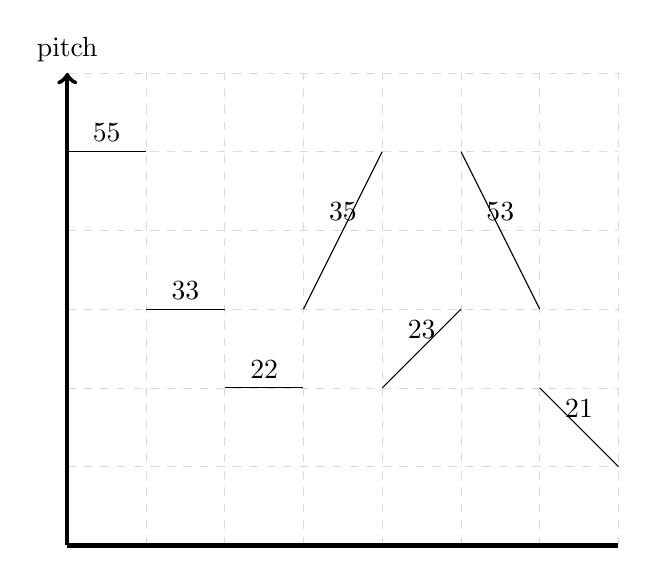
\begin{tikzpicture}
\draw [help lines, color=gray!30, dashed] (0, 0) grid (7, 6);
\draw [->, ultra thick] (0, 0) -- (0, 6) node [above]{pitch};
\draw [ultra thick] (0, 0) -- (7, 0);
\draw (0, 5) -- node [above]{55} (1, 5);
\draw (1, 3) -- node [above]{33} (2, 3);
\draw (2, 2) -- node [above]{22} (3, 2);
\draw (3, 3) -- node [above]{35} (4, 5);
\draw (4, 2) -- node [above]{23} (5, 3);
\draw (5, 5) -- node [above]{53} (6, 3);
\draw (6, 2) -- node [above]{21} (7, 1);
\end{tikzpicture}

\renewcommand{\arraystretch}{2}
\begin{tabularx}{\linewidth}{l l l l}
    high level & :55 & \jping{si1} & 詩 \\
    mid level & :33 & \jping{si3} & 試 \\
    low level & :22 & \jping{si6} & 事 \\
    high rising & :35 & \jping{si2} & 史 \\
    low rising & :23 & \jping{si5} & 市 \\
    high falling & :53 & \jping{si7} & 思 \\
    low falling & :21 & \jping{si4} & 時 \\
\end{tabularx}
\renewcommand{\arraystretch}{1}

\end{minipage}

\begin{minipage}{\linewidth}

In present day Standard Cantonese as spoken in Hong Kong the high falling tone seems to be dying out. Many people do not have a high falling tone in their speech, and use high level tones in place of high falling. These people have just six tones in their speech. In this book we mark seven tones, but your teacher may only have six, and the tapes accompanying the text include the speech of some speakers with only six tones. Copy what you hear. High falling and high level tones are given in the examples below. If you do not hear a difference, your teacher doesn't differentiate.

\audioTag{A}{15:56}

Ex: high-falling, high-level contrasts
\renewcommand{\arraystretch}{2}
\begin{tabularx}{\linewidth}{l l l l}
    1. & \jping{saam7} & three & 三 \\
       & \jping{saam1} & clothing & 衫 \\
    2. & \jping{fan7} & divide & 分 \\
       & \jping{fan1} & minute & 分 \\
    3. & \jping{ho4saang7} & Mr. Ho & 何生 \\
       & \jping{hok6saang1} & student & 學生 \\
    4. & \jping{si7} & think & 思 \\
       & \jping{si1} & poetry & 詩 \\
\end{tabularx}
\renewcommand{\arraystretch}{1}

\end{minipage}

%%%%%%%%%%%%%%%%%%%%%%%%%%%%%%%%%%%%%%%%
\begin{minipage}{\linewidth}

\paragraph{Tonal Spelling}

The system of tonal spelling we will use in this book is a modified form of the Huang-Kok yale romanization. This system divides the tones into two group, an upper register group and a lower register one. The lower register tones are marked by an \underline{h} following the vowel of the syllable. This \underline{h} is silent and simply indicates lower register. The upper register group doesn't have the \underline{h}

\audioTag{A}{16:14}

Ex: Upper register tones
\renewcommand{\arraystretch}{2}
\begin{tabularx}{\linewidth}{l l l}
    \jping{si1} & sī & 詩 \\
    \jping{si7} & sì & 思 \\
    \jping{si2} & sí & 史 \\
    \jping{si3} & si & 試 \\
\end{tabularx}
\renewcommand{\arraystretch}{1}

\audioTag{A}{16:23}

Ex: Lower register tones
\renewcommand{\arraystretch}{2}
\begin{tabularx}{\linewidth}{l l l}
    \jping{si4} & sìh & 時 \\
    \jping{si5} & síh & 市 \\
    \jping{si6} & sih & 事 \\
\end{tabularx}
\renewcommand{\arraystretch}{1}

The rising, falling, and level contours of the tones are indicated by the presence or absence of diacritics over the vowel of each syllable. The diacritics `, ´, ¯ representing falling, rising, and level respectively.

\renewcommand{\arraystretch}{2}
\begin{tabularx}{\linewidth}{l l}
    à & falling \\
    á & rising \\
    ā & level \\
\end{tabularx}
\renewcommand{\arraystretch}{1}

The absence of a diacritic represents level tone.

\renewcommand{\arraystretch}{2}
\begin{tabularx}{\linewidth}{l l}
    a & \\
\end{tabularx}
\renewcommand{\arraystretch}{1}

\end{minipage}

\begin{minipage}{\linewidth}

Using three diacritics and the low register symbol \underline{h}, we spell the seven tones thus:

\renewcommand{\arraystretch}{2}
\begin{tabularx}{\linewidth}{l l l}
    \jping{a1} & ā & high level \\
    \jping{a3} & a & mid level \\
    \jping{a6} & ah & low level \\
    \jping{a7} & à & high falling \\
    \jping{a4} & àh & low falling \\
    \jping{a2} & á & high rising \\
    \jping{a5} & áh & low rising \\
\end{tabularx}
\renewcommand{\arraystretch}{1}

\end{minipage}

\begin{minipage}{\linewidth}

The low register symbol \underline{h} follows the vowel of the syllable. If the syllable ends with a consonant, the \underline{h} still follows the vowel, but comes before the final consonant.

\audioTag{A}{16:29}

\renewcommand{\arraystretch}{2}
\begin{tabularx}{\linewidth}{l l l}
    \jping{sap6} & sahp & ten \\
    \jping{seng4} & sèhng & whole, entire \\
\end{tabularx}
\renewcommand{\arraystretch}{1}

\end{minipage}

\begin{minipage}{\linewidth}

Traditionally Chinese recite Cantonese tones in upper register - lower register sequence, in the order falling, rising, level, thus.

\audioTag{A}{16:37}

\renewcommand{\arraystretch}{2}
\begin{tabularx}{\linewidth}{l l l}
    \jping{si7} & 思 & 53 \\
    \jping{si2} & 史 & 35 \\
    \jping{si3} & 試 & 33 \\
    \jping{si4} & 時 & 21 \\
    \jping{si5} & 市 & 23 \\
    \jping{si6} & 事 & 22 \\
\end{tabularx}
\renewcommand{\arraystretch}{1}

\centering
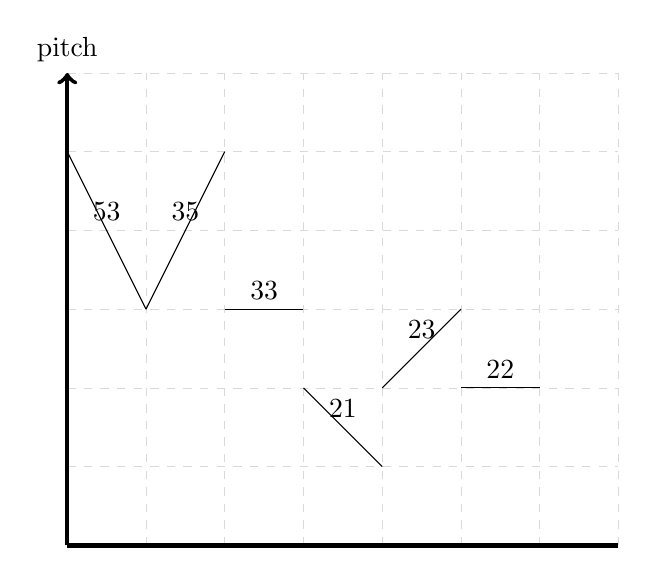
\begin{tikzpicture}
\draw [help lines, color=gray!30, dashed] (0, 0) grid (7, 6);
\draw [->, ultra thick] (0, 0) -- (0, 6) node [above]{pitch};
\draw [ultra thick] (0, 0) -- (7, 0);
\draw (0, 5) -- node [above]{53} (1, 3);
\draw (1, 3) -- node [above]{35} (2, 5);
\draw (2, 3) -- node [above]{33} (3, 3);
\draw (3, 2) -- node [above]{21} (4, 1);
\draw (4, 2) -- node [above]{23} (5, 3);
\draw (5, 2) -- node [above]{22} (6, 2);
\end{tikzpicture}

This is the way Cantonese themselves recite tones. You will note that the high level tone is not recieted traditionally. There are historical reasons for this which we won't go into here.

\end{minipage}

\begin{minipage}{\linewidth}

In a few words the consonants \underline{m} and \underline{ng} occur as vowels, and in this cases the diacritics are places above the \underline{n} of \underline{ng} and the \underline{m}.

\audioTag{A}{16:52}

\renewcommand{\arraystretch}{2}
\begin{tabularx}{\linewidth}{l l l}
    \jping{m4} & m̀h & not \\
    \jping{ng5} & ńgh & five \\
\end{tabularx}
\renewcommand{\arraystretch}{1}

\end{minipage}

%%%%%%%%%%%%%%%%%%%%%%%%%%%%%%%%%%%%%%%%
\begin{minipage}{\linewidth}

\paragraph{Tones in Sequence}

\underline{Tone Sandhi}. Changes in the basic sound of tones when syllables are spoken in sequence is called tone sandhi. The high falling tone in Cantonese undergoes tone sandhi in certain position, as follows:

\audioTag{A}{17:03}

1. When high falling tones occur in succession without intervening pause, all but the final ones are pronounced as high level:

Ex: hf + hf becomes hl + hf

\renewcommand{\arraystretch}{2}
\begin{tabularx}{\linewidth}{X X X}
roast pig (roast pork) & \dtext{燒豬}{siu7zyu7} & \dtext{燒豬}{siu1zyu7} \\
hurt wind (to catch cold) & \dtext{傷風}{soeng7fung7} & \dtext{傷風}{soeng1fung7} \\
hurt wind tim! (hurt wind!), caught cold! & \dtext{傷風添}{soeng7fung7tim7} & \dtext{傷風添}{soeng1fung1tim7} \\
\end{tabularx}
\renewcommand{\arraystretch}{1}

\audioTag{A}{17:43}

2. When a high falling tone occurs before a high level tone without intervening pause, it is pronounced as high level.

Ex: hf + hl becomes hl + hl

\renewcommand{\arraystretch}{2}
\begin{tabularx}{\linewidth}{X X X}
rent house (to rent a house) & \dtext{租屋}{zou7uk1} & \dtext{租屋}{zou1uk1} \\
west meal (western food) & \dtext{西餐}{sai7caan1} & \dtext{西餐}{sai1caan1} \\
\end{tabularx}
\renewcommand{\arraystretch}{1}

In this book high falling tone has been written high level only when the tone sandhi is within word boundaries. For separate words, the high falling will be marked with its usual diacritic.

\renewcommand{\arraystretch}{2}
\begin{tabularx}{\linewidth}{X X X}
first born (man, teacher, Mr.) & \dtext{先生}{sin7saang7} & \dtext{先生}{sin1saang7} \\
Cheung Mr. (Mr. Cheung) & \dtext{張生}{zoeng7saang7} & \dtext{張生}{zoeng7saang7} \\
\end{tabularx}
\renewcommand{\arraystretch}{1}

\end{minipage}

%%%%%%%%%%%%%%%%%%%%%%%%%%%%%%%%%%%%%%%%
\paragraph{Tones not 'sung'}

That Cantonese is a tone language does not mean that sentences in it are sung as you would sign a medical phrase. Music has sustained notes and strict rhythmic scheme, the spoken language does not. At first you may feel that Cantonese sounds sing-song, but practice will bring familiarity and soon it will sound natural to you.
\subsubsection{Intonation}

A sentence may be said different ways, to stress different points in the sentence and also to express what the speaker feels about what he is saying. To give an English example, the sentence 'So glad you could come', may be said:

\todo{contour graphs}

\begin{tabularx}{\linewidth}{X X X}
So glad you could \underline{come}. &
\begin{tikzpicture}
\draw (0, 0) -- (3, 0);
\draw (3, 0) -- (4, 0.5);
\draw [->] (4, 0.5) -- (4.5, 0);
\end{tikzpicture}
& normal polite \\

\underline{So} glad you could come. &
\begin{tikzpicture}
\draw (0, 0.5) -- (1, 0);
\draw (1, 0) -- (4, 0);
\draw [->] (4, 0) -- (4.5, -0.5);
\end{tikzpicture}
& effusive polite \\

So glad \underline{you} could come. &
\begin{tikzpicture}
\draw (0, 0) -- (1, 0);
\draw (1, 0) -- (2, 0.5);
\draw (2, 0.5) -- (3, 0);
\draw (3, 0) -- (4, 0);
\draw [->] (4, 0) -- (4.5, -0.5);
\end{tikzpicture}
& (even if your wife couldn't make it) cordial \\

So glad \underline{you} could come. &
\begin{tikzpicture}
\draw (0, 0) -- (1, 0);
\draw (1, 0) -- (2, 0.75);
\draw (2, 0.75) -- (3, 0);
\draw (3, 0) -- (4, 0);
\draw [->] (4, 0) -- (4.5, -0.5);
\end{tikzpicture}
& (even if your \underline{wife} couldn't) sarcastic \\

So glad you \underline{could} come. &
\begin{tikzpicture}
\draw (0, 0) -- (2, 0);
\draw (2, 0) -- (3, 0.5);
\draw [->] (3, 0.5) -- (4.5, -0.5);
\end{tikzpicture}
& (after having though you couldn't) cordial \\

They were glad you could come? &
\begin{tikzpicture}
\draw (0, 0) -- (4, 0);
\draw (4, 0) -- (4.5, 0.5);
\draw [->] (4.5, 0.5) -- (5, 1);
\end{tikzpicture}
& question \\
\end{tabularx}

The graphs of the sentence contours above represent the rise and fall of the voice pitch throughout the length of the sentence. This rise and fall over sentence length we call and "intonation".

You will note that the question sentence (\#5) rises in pitch at the end, and the statement sentences (\#1 - 4) all end with falling pitch, although within their contours rise and fall occurs at different points. In English sentence-final fall is the norm, and sentence-final expresses doubt.

Intonation asl has another job within a sentence, it can express how the speaker feels about what he is saying. By expressive rise and fall of his voice, by varying his "tone of voice", the speaker can indicate that he is angry or happy, doubtful or certain, being polite or rude, suggesting or demanding.

Cantonese sentences too exhbiti intonation contours. Sentence final contours in particular are much more varied in Cantonese than in English, and capable of expressing quite a range of emotional implications.

You may wonder how intonation affects the tone situation in Cantonese, each syllable having as it done its characteristic tone. How the tone contours operate in the framework of sentence contour has been compared to the action of ripples riding on top of waves. Each ripple relates to the one before it and behind it, whether in the trough of the wave or on the crest.

%%%%%%%%%%%%%%%%%%%%%%%%%%%%%%%%%%%%%%%%%%%%%%%%%%%%%%%%%%%%%%%%%%%%%%%%%%%%%%%%
\paragraph{Sentence Stress}

In speaking of sentence stress we mean relative prominence of syllables in a sentence - loud or soft (heavy or light), rapid or slow. Consider the stress pattern of the following English sentences.

\begin{tabularx}{\linewidth}{X X X}
\underline{I'm} John Smith. & (In response to "Which one of you is John Smith?") \\
I'm \underline{John} Smith. & (In response to "I was suppsed to give this letter to Tom Smith") \\
\end{tabularx}

In the sentence above the stressed syllables (those underlined) give prominence to the information requested in the stimulus sentences.

In certain sentences stress differences alone indicate dfference in message content. The pair of sentences often quoted in illustration of this is:

\begin{tabularx}{\linewidth}{X X X}
\underline{Ship} sails today. && (The ship will sail today.) \\
Ship \underline{sails} today. && (Please ship the sails today.) \\
\end{tabularx}

Another example, from a headline in a newspaper:
\indent Boy Scratching Cat is Caught, Destroyed
How do you stress that one?

%%%%%%%%%%%%%%%%%%%%%%%%%%%%%%%%%%%%%%%%%%%%%%%%%%%%%%%%%%%%%%%%%%%%%%%%%%%%%%%%
\paragraph{Sentence Pause}

Another feature important in establishing natural sentence rhythm is pause - the small silences between groups of syllables. Note the following English sentence:

\begin{quote}
	In considering him for the job he took into account his education, previous experience, and appraised potential.
\end{quote}

There is a pause between "job" and "he" in the sentence above, and if you read it instead pausing after "took", you find the sentence doesn't make sense - you have to go back and read it again putting a pause in the right place.

We will not discuss Cantonese stress and pause features in this Introduction, other than to say that Cantonese sentences, like English ones, do exhibit stress and pause phenomena, as well as intonational ones. What this effectively means for you as a student is that you must not concentrate solely on learning words as individual isolated units, but in imitating the teacher's spoken model, you should be alert to his delivery of prhase-length segments and whole sentences, and should mimic the stress, pause, and intonation of the phrases you repeat.

\subsubsection{Consonants and Vowels}
\todo{copy}

\subsection{Pronounciation Practice}
\todo{copy}
\subsection{Culture Notes}
\todo{copy}
\subsection{Drills}

%%%%%%%%%%%%%%%%%%%%%%%%%%%%%%%%%%%%%%%%

\begin{minipage}{\linewidth}

\paragraph{1. Subsitution Drill} Substitute \dtext{再見}{zoi3gin3} in the position of \dtext{早晨}{zou2san4} following the pattern of the example sentence.

\drillExample{
    \drillExampleEntry {T} {\dtext{李 太,早晨}{lei5 taai2 zou2san4}} {Good morning, Mrs. Lee.}
    \drillExampleEntry {S} {\dtext{李 太,再見}{lei5 taai2 zoi3gin3}} {Goodbye, Mrs. Lee.}
}

\drill{
    \drillEntry {1} {\dtext{陳 太,早晨}{can4 taai2 zou2san4}}{\dtext{陳 太,再見} {can4 taai2 zoi3gin3}}
    \drillEntryTrans {Good morning, Miss Chan.} {}
    %
    \drillEntry {2} {\dtext{劉 生,早晨}{lau4 saang1 zou2san4}}{\dtext{劉 生,再見} {lau4 saang1 zoi3gin3}}
    \drillEntryTrans {Good morning, Mr. Lau.} {}
    %
    \drillEntry {3} {\dtext{張 小姐,早晨}{zoeng1 siu2ze2 zou2san4}}{\dtext{張 小姐,再見} {zoeng1 siu2ze2 zoi3gin3}}
    \drillEntryTrans {Good morning, Miss Cheung.} {}
    %
    \drillEntry {4} {\dtext{馬 生,早晨}{maa5 saang1 zou2san4}}{\dtext{馬 生,再見} {maa5 saang1 zoi3gin3}}
    \drillEntryTrans {Good morning, Mr. Ma.} {}
    %
    \drillEntry {5} {\dtext{李 太,早晨}{lei5 taai2 zou2san4}}{\dtext{李 太,再見}{lei5 taai2 zoi3gin3}}
    \drillEntryTrans {Good morning, Miss Lee.} {}
}

\end{minipage}

%%%%%%%%%%%%%%%%%%%%%%%%%%%%%%%%%%%%%%%%%%%%%%%%%%%%%%%%%%%%%%%%%%%%%%%%%%%%%%%%

\begin{minipage}{\linewidth}

\paragraph{2. Subsitution Drill} Substitute the cue in the appropriate position following the pattern of the example sentence.

\drillExample{
    \drillExampleEntrySub {T} {\dtext{李 太,早晨}{lei5 taai2 zou2san4}} {Good morning, Mrs. Lee.} {\dtext{陳}{can4}}
    \drillExampleEntry {S} {\dtext{陳 太,再見}{can4 taai2 zoi3gin3}} {Good morning, Mrs. Chan.}
}

\drill{
    \drillEntrySub {1} {\dtext{陳 太,早晨}{can4 taai2 zou2san4}} {\dtext{李 太,早晨}{lei5 taai2 zou2san4}} {\dtext{李}{lei5}}
    \drillEntrySub {2} {\dtext{李 太,早晨}{lei5 taai2 zou2san4}} {\dtext{王 太,早晨}{wong4 taai2 zou2san4}} {\dtext{王}{wong4}}
    \drillEntrySub {3} {\dtext{王 太,早晨}{wong4 taai2 zou2san4}} {\dtext{何 太,早晨}{ho4 taai2 zou2san4}} {\dtext{何}{ho4}}
    \drillEntrySub {4} {\dtext{何 太,早晨}{ho4 taai2 zou2san4}} {\dtext{張 太,早晨}{zoeng1 taai2 zou2san4}} {\dtext{張}{zoeng1}}
    \drillEntrySub {5} {\dtext{劉 太,早晨}{lau4 taai2 zou2san4}} {\dtext{陳 太,早晨}{can4 taai2 zou2san4}} {\dtext{陳}{can4}}
}

\end{minipage}

%%%%%%%%%%%%%%%%%%%%%%%%%%%%%%%%%%%%%%%%%%%%%%%%%%%%%%%%%%%%%%%%%%%%%%%%%%%%%%%%

\begin{minipage}{\linewidth}

\paragraph{3. Subsitution Drill} Substitute the cue in the appropriate position, following the pattern of the example sentence.

\drillExample{
    \drillExampleEntrySub {T} {\dtext{王 生,早晨}{wong4 saang1 zou2san4}} {Good morning, Mr. Wong.} {\dtext{太}{taai2}}
    \drillExampleEntry {S} {\dtext{王 太,早晨}{wong4 taai2 zou2san4}} {Good morning, Mrs. Wong.}
}

\drill{
    \drillEntrySub {1} {\dtext{王 太,早晨}{wong4 taai2 zou2san4}} {\dtext{王 小姐,早晨}{wong4 siu2ze2 zou2san4}} {\dtext{小姐}{siu2ze2}}
    \drillEntrySub {2} {\dtext{王 小姐,早晨}{wong4 siu2ze2 zou2san4}} {\dtext{劉 小姐,早晨}{lau4 siu2ze2 zou2san4}} {\dtext{劉}{lau4}}
    \drillEntrySub {3} {\dtext{劉 小姐,早晨}{lau4 siu2ze2 zou2san4}} {\dtext{劉 小姐,再見}{lau4 siu2ze2 zoi3gin3}} {\dtext{再見}{zoi3gin3}}
    \drillEntrySub {4} {\dtext{劉 小姐,再見}{lau4 siu2ze2 zoi3gin3}} {\dtext{劉 生,再見}{lau4 saang1 zoi3gin3}} {\dtext{生}{saang1}}
    \drillEntrySub {5} {\dtext{劉 生,再見}{lau4 saang1 zoi3gin3}} {\dtext{劉 太,再見}{lau4 taai2 zoi3gin3}} {\dtext{太}{taai2}}
}

\end{minipage}

%%%%%%%%%%%%%%%%%%%%%%%%%%%%%%%%%%%%%%%%%%%%%%%%%%%%%%%%%%%%%%%%%%%%%%%%%%%%%%%%

\begin{minipage}{\linewidth}

\paragraph{4. Expansion Drill} Expand the cue sentance as indicated in the example.

\drillExample{
    \drillExampleEntry {T} {\dtext{我 唔係 王 生}{ngo5 m4hai6 wong4 saang1}} {I'm not Mr. Wong.}
    \drillExampleEntry {S} {\dtext{對唔住 我 唔係 王 生}{deoi3m4zyu6 ngo5 m4hai6 wong4 saang1}}
}

\drill{
    \drillEntry {1} {\dtext{我 唔係 李 小姐}{ngo5 m4hai6 lei5 sui2ze2}} {\dtext{對唔住,我 唔係 李 小姐}{deoi3m4zyu6 ngo5 m4hai6 lei5 sui2ze2}}
    \drillEntry {2} {\dtext{我 唔係 陳 生}{ngo5 m4hai6 can4 saang1}} {\dtext{對唔住,我 唔係 陳 生}{deoi3m4zyu6 ngo5 m4hai6 can4 saang1}}
    \drillEntry {3} {\dtext{我 唔係 張 太}{ngo5 m4hai6 zoeng1 taai2}} {\dtext{對唔住,我 唔係 張 太}{deoi3m4zyu6 ngo5 m4hai6 zoeng1 taai2}}
    \drillEntry {4} {\dtext{我 唔係 何 生}{ngo5 m4hai6 ho4 saang1}} {\dtext{對唔住,我 唔係 何 生}{deoi3m4zyu6 ngo5 m4hai6 ho4 saang1}}
    \drillEntry {5} {\dtext{我 唔係 王 太}{ngo5 m4hai6 wong4 taai2}} {\dtext{對唔住,我 唔係 王 太}{deoi3m4zyu6 ngo5 m4hai6 wong4 taai2}}
}

\end{minipage}

%%%%%%%%%%%%%%%%%%%%%%%%%%%%%%%%%%%%%%%%%%%%%%%%%%%%%%%%%%%%%%%%%%%%%%%%%%%%%%%%

\begin{minipage}{\linewidth}

\paragraph{5. Expansion Drill} Expand the cue sentance to conform with the pattern of the example.

\drillExample{
    \drillExampleEntrySub {T} {\dtext{我 唔係 李 太}{ngo5 m4hai6 lei5 taai2}}{I'm not Mrs. Lee} {\dtext{}{zoeng1}}
    \drillExampleEntry {S} {\dtext{我 唔係 李 太,我 姓 張}{ngo5 m4hai6 lei5 taai2 ngo5 sing3 zoeng1}} {I'm not Mrs. Lee, my name is Cheung.}
}

\drill{
    \drillEntrySub {1} {\dtext{我 唔係 何 太}{ngo5 m4hai6 ho4 taai2}} {\dtext{我 唔係 何 太,我 姓 陳}{ngo5 m4hai6 ho4 taai ngo5 sing3 can4}} {\dtext{陳}{can4}}
    \drillEntrySub {2} {\dtext{我 唔係 陳 小姐}{ngo5 m4hai6 can4 siu2ze2}} {\dtext{我 唔係 陳 小姐,我 姓 馬}{ngo5 m4hai6 can4 siu2ze2 ngo5 sing3 maa5}} {\dtext{馬}{maa5}}
    \drillEntrySub {3} {\dtext{我 唔係 馬 生}{ngo5 m4hai6 maa5 saang1}} {\dtext{我 唔係 馬 生,我 姓 王}{ngo5 m4hai6 maa5 saang1 ngo5 sing3 wong4}} {\dtext{王}{wong4}}
    \drillEntrySub {4} {\dtext{我 唔係 王 太}{ngo5 m4hai6 wong4 taai2}} {\dtext{我 唔係 王 太,我 姓 張}{ngo5 m4hai6 wong4 taai2 ngo5 sing3 zoeng1}} {\dtext{張}{zoeng1}}
    \drillEntrySub {5} {\dtext{我 唔係 李 太}{ngo5 m4hai6 lei5 taai2}} {\dtext{我 唔係 李 太,我 姓 }{ngo5 m4hai6 lei5 taai2 ngo5 sing3 ho4}} {\dtext{何}{ho4}}
}

\end{minipage}

%%%%%%%%%%%%%%%%%%%%%%%%%%%%%%%%%%%%%%%%%%%%%%%%%%%%%%%%%%%%%%%%%%%%%%%%%%%%%%%%

\paragraph{6. Conversation Drill} Carry on the suggested conversation following the model of the example.

\drillExample{
    \drillExampleEntry {A} {\dtext{陳 生, 早晨。}{can4 saang1 zou2san4}} {Good morning Mr. Chan.}
    \drillExampleEntry {B} {\dtext{對唔住,我 唔係 陳 生。我 姓 張。}{deoi3m4zyu6 ngo5 m4hai6 can4 saang1 ngo5 sing3 zoeng1}} {I beg your pardon, I'm not Mr. Chan. My name is Cheung.}
    \drillExampleEntry {A} {\dtext{呀,對唔住,張 生。}{aa3 deoi3m4zyu6 zoeng1 sang1}} {A, excuse me, Mr. Cheung.}
    \drillExampleEntry {B} {\dtext{唔緊要。}{m4gan2jiu3}} {That's OK.}
}

\convDrill{
    \convDrillEntry {1} {A} {\dtext{陳 小姐}{can4 siu2ze2} ... } {\dtext{陳 小姐 早晨。}{can4 siu2ze2 jou2san4}}
    \convDrillEntry {} {B} { ... \dtext{王}{wong4}} {\dtext{對唔住,我 唔係 陳 小姐。我 姓 王。}{deoi3m4zyu6 ngo5 m4hai6 can4 siu2ze2 ngo5 sing3 wong4}}
    \convDrillEntry {} {A} { ... } {\dtext{呀 對唔住 王 小姐。}{aa3 deoi3m4zyu6 wong4 siu2ze2}}
    \convDrillEntry {} {B} { ... } {\dtext{唔緊要。}{m4gan2jiu3}}
    %
    \convDrillEntry {2} {A} {\dtext{張 小姐}{zoeng1 siu2ze2} ... } {\dtext{張 小姐 早晨。}{zoeng1 siu2ze2 jou2san4}}
    \convDrillEntry {} {B} { ... \dtext{李}{lei5}} {\dtext{對唔住,我 唔係 張 小姐。我 姓 李。}{deoi3m4zyu6 ngo5 m4hai6 zoeng1 siu2ze2 ngo5 sing3 lei5}}
    \convDrillEntry {} {A} { ... } {\dtext{呀 對唔住 李 小姐。}{aa3 deoi3m4zyu6 lei5 siu2ze2}}
    \convDrillEntry {} {B} { ... } {\dtext{唔緊要。}{m4gan2jiu3}}
    %
    \convDrillEntry {3} {A} {\dtext{何 生}{ho4 saang1} ... } {\dtext{何 生 早晨。}{ho4 saang1 jou2san4}}
    \convDrillEntry {} {B} { ... \dtext{王}{wong4}} {\dtext{對唔住,我 唔係 何 生。我 姓 王。}{deoi3m4zyu6 ngo5 m4hai6 ho4 saang1 ngo5 sing3 wong4}}
    \convDrillEntry {} {A} { ... } {\dtext{呀 對唔住 王 生。}{aa3 deoi3m4zyu6 wong4 saang1}}
    \convDrillEntry {} {B} { ... } {\dtext{唔緊要。}{m4gan2jiu3}}
    %
    \convDrillEntry {4} {A} {\dtext{張 小姐}{zoeng1 saang1} ... } {\dtext{張 小姐 早晨。}{zoeng1 saang1 jou2san4}}
    \convDrillEntry {} {B} { ... \dtext{李}{wong4}} {\dtext{對唔住,我 唔係 張 小姐。我 姓 李。}{deoi3m4zyu6 ngo5 m4hai6 zoeng1 saang1 ngo5 sing3 wong4}}
    \convDrillEntry {} {A} { ... } {\dtext{呀 對唔住 李 小姐。}{aa3 deoi3m4zyu6 wong4 saang1}}
    \convDrillEntry {} {B} { ... } {\dtext{唔緊要。}{m4gan2jiu3}}
    %
    \convDrillEntry {5} {A} {\dtext{陳 小姐}{can4 siu2ze2} ... } {\dtext{陳 小姐 早晨。}{can4 siu2ze2 jou2san4}}
    \convDrillEntry {} {B} { ... \dtext{劉}{lau4}} {\dtext{對唔住,我 唔係 陳 小姐。我 姓 劉。}{deoi3m4zyu6 ngo5 m4hai6 can4 siu2ze2 ngo5 sing3 lau4}}
    \convDrillEntry {} {A} { ... } {\dtext{呀 對唔住 劉 小姐。}{aa3 deoi3m4zyu6 lau4 siu2ze2}}
    \convDrillEntry {} {B} { ... } {\dtext{唔緊要。}{m4gan2jiu3}}
}

\subsection{Vocabulary Checklist}

\vocabularyChecklist{
    {\dtext{呀}{aa3}}
    {ex}
    {Oh}
    %
    {\dtext{陳}{can4}}
    {sur}
    {Chan}
    %
    {\dtext{對唔住}{deoi3m4zyu6}}
    {ph}
    {Excuse me; I beg your pardon; I'm sorry.}
    %
    {\dtext{係}{hai6}}
    {v}
    {is, am, are, were, etc.}
    %
    {\dtext{何}{ho4}}
    {sur}
    {Ho}
    %
    {\dtext{學生}{hok6saang1}}
    {n}
    {student}
    %
    {\dtext{張}{zoeng1}}
    {sur}
    {Cheung}
    %
    {\dtext{再見}{zoi3gin3}}
    {ph}
    {Goodbye}
    %
    {\dtext{早晨}{zou2san4}}
    {ph}
    {Good morning}
    %
    {\dtext{劉}{lau4}}
    {sur}
    {Lau}
    %
    {\dtext{李}{lei5}}
    {sur}
    {Li (Lee)}
    %
    {\dtext{馬}{maa5}}
    {sur}
    {Ma}
    %
    {\dtext{唔-}{m4}}
    {adv}
    {not}
    %
    {\dtext{唔緊要}{m4gan2jiu3}}
    {ph}
    {That's all right; It doesn't matter; Never mind.}
    %
    {\dtext{我}{ngo5}}
    {pro}
    {I, me, my}
    %
    {\dtext{生}{saang1}}
    {t}
    {Mr.}
    %
    {\dtext{先生}{sin1saang1}}
    {n}
    {Man (see notes); teacher}
    %
    {\dtext{先生}{sin1saang1}}
    {t}
    {Mr. (see notes)}
    %
    {\dtext{姓}{sing3}}
    {v}
    {to have the surname}
    %
    {\dtext{小姐}{siu2ze2}}
    {n}
    {unmarried woman; womand, lady (see notes)}
    %
    {\dtext{小姐}{siu2ze2}}
    {t}
    {Miss.}
    %
    {\dtext{太}{taai2}}
    {t}
    {Mrs.}
    %
    {\dtext{太太}{taai3taai2}}
    {n}
    {married woman (see notes)}
    %
    {\dtext{太太}{taai3taai2}}
    {t}
    {Mrs. (see notes)}
    %
    {\dtext{王}{wong4}}
    {sur}
    {Wong}
    %
}



\end{document}